\section{Free Functions in the Arrangement Package\label{arr_sec:gl_funcs}}
%==================================================

In Section~\ref{arr_sec:arr_class} we reviewed in details the
\ccc{Arrangement_2} class, which represents two-dimensional
subdivisions induced by planar curves, and mentioned that its
interface is minimal in the sense that the member functions hardly
perform any geometric algorithms and are mainly used for
maintaining the topological structure of the subdivision. In this
section we explain how to utilize the free (global) functions that operate
on arrangements. The implementation of these operations typically require
non-trivial geometric algorithms or load some extra requirements on
the traits class.

\subsection{Incremental Insertion Functions\label{arr_ssec:inc_insert}}
%-------------------------------------------

\subsubsection{Inserting Non-Intersecting Curves\label{arr_sssec:insert_non_x}}
%~~~~~~~~~~~~~~~~~~~~~~~~~~~~~~~~~~~~~~~~~~~~~~~~

In Section~\ref{arr_sec:arr_class} we explained how to construct
arrangements of $x$-monotone curves that are pairwise disjoint in
their interior, when the location of the segment endpoints in the
arrangement is known. Here we relax this constraint, and allow the
location of the inserted $x$-monotone curve endpoints to be arbitrary,
as it may be unknown at the time of insertion. We retain, for the moment,
the requirement that the interior of the inserted curve is disjoint from
all existing arrangement edges and vertices.

The free function \ccc{insert_non_intersecting_curve(arr, c, pl)}
inserts the $x$-monotone curve $c$ into the arrangement \ccc{arr},
with the precondition that the interior of $c$ is disjoint from
all \ccc{arr}'s existing edges and vertices. The third argument
\ccc{pl} is a point-location object attached to the arrangement,
which is used for performing the insertion. It locates both curve
endpoints in the arrangement, where each endpoint is expected to
either coincide with an existing vertex or lie inside a face.
It is possible to invoke one of the specialized insertion functions
(see Section~\ref{arr_sec:arr_class}), based on the query results, and
insert $c$ at its proper position.\footnote{The
\ccc{insert_non_intersecting_curve()} function, as all other functions
reviewed in this section, is a function template, parameterized by an
arrangement class and a point-location class (a model of the
\ccc{ArrangementPointLocation_2} concept).} The insertion operation
thus hardly requires any geometric operations on top on the ones
needed to answer the point-location queries. Moreover, it is
sufficient that the arrangement class is instantiated with a
traits class that models the \ccc{ArrangementBasicTraits_2}
concept (or the \ccc{ArrangementLandmarkTraits_2} concept, if the
landmark point-location strategy is used), which does not have to
support the computation of intersection points between curves.

The variant \ccc{insert_non_intersecting_curve(arr, c)} is also
available. Instead of accepting a user-defined point-location
object, it defines a local instance of the walk point-location
class and uses it to insert the curve.

\subsubsection{Inserting $x$-Monotone Curves\label{arr_sssec:insert_x_mon}}
%~~~~~~~~~~~~~~~~~~~~~~~~~~~~~~~~~~~~~~~~~~~~

The \ccc{insert_non_intersecting_curve()} function is very
efficient, but its preconditions on the input curves are still
rather restricting. Let us assume that the arrangement is
instantiated with a traits class that models the refined
\ccc{ArrangementXMonotoneTraits_2} concept and supports
intersection computations (see Section~\ref{arr_sec:traits} for
the exact details). Given an $x$-monotone curve, it is sufficient
to locate its left endpoint in the arrangement and to trace its
{\em zone}, namely the set of arrangement features crossing the curve,
until the right endpoint is reached. Each time the new curve $c$
crosses an existing vertex or an edge, the curve is split into
subcurves (in the latter case, we have to split the curve 
associated with the existing halfedge as well) and associate new
edges with the resulting subcurves. Recall that an edge is represented
by a pair of twin halfedges, so we split it into two halfedge pairs.

The free function \ccc{insert_x_monotone_curve(arr, c, pl)} performs
this insertion operation. It accepts an $x$-monotone curve $c$,
which may intersect some of the curves already in the arrangement
\ccc{arr}, and inserts it into the arrangement by computing its zone.
Users may supply a point-location object \ccc{pl}, or use the default
walk point-location strategy (namely, the variant
\ccc{insert_x_monotone_curve(arr, c)} is also available). The
running-time of this insertion function is proportional to the
complexity of the zone of the curve $c$.

\begin{ccAdvanced}
In some cases users may have a prior knowledge of the location of the
left endpoint of the $x$-monotone curve \ccc{c} they wish to insert,
so they can perform the insertion without issuing any point-location
queries. This can be done by calling
\ccc{insert_x_monotone_curve(arr, c, obj)}, where \ccc{obj} is an
object represents the location of \ccc{c}'s left endpoint in the
arrangement --- namely it wraps a \ccc{Vertex_const_handle}, a
\ccc{Halfedge_const_handle} or a \ccc{Face_const_handle} (see
also Section~\ref{arr_ssec:pl}).
\end{ccAdvanced}

\subsubsection{Inserting General Curves\label{arr_sssec:insert_gen}}
%~~~~~~~~~~~~~~~~~~~~~~~~~~~~~~~~~~~~~~~

So far all our examples were of arrangements of line segments,
where the \ccc{Arrangement_2} template was instantiated with the
\ccc{Arr_segment_traits_2} class. In this case, the fact that
\ccc{insert_x_monotone_curve()} accepts an $x$-monotone curve does not
seem to be a restriction, as all line segments are $x$-monotone
(note that we consider vertical line segments to be {\em weakly}
$x$-monotone).

Suppose that we construct an arrangement of circles. A circle is
obviously not $x$-monotone, so we cannot use
\ccc{insert_x_monotone_curve()} in this case.\footnote{Note that a key
operation performed by \ccc{insert_x_monotone_curve()} is to locate the
left endpoint of the curve in the arrangement. A circle, however, does
not have any endpoints!} However, it is possible to subdivide each circle
into two $x$-monotone circular arcs (its upper half and its lower
half) and to insert each $x$-monotone arc separately.

The free function \ccc{insert_curve()} requires that the traits class
used by the arrangement \ccc{arr} to be a model of the concept
\ccc{ArrangementTraits_2}, which refines the
\ccc{ArrangementXMonotoneTraits_2} concept. It has to define an
additional \ccc{Curve_2} type (which may differ from the
\ccc{X_monotone_curve_2} type), and support the subdivision of curves
of this new type into $x$-monotone curves (see the exact details in
Section~\ref{arr_sec:traits}). The \ccc{insert_curve(arr, c, pl)}
function performs the insertion of the curve $c$, which does not need
to be $x$-monotone, into the arrangement by subdividing it into
$x$-monotone subcurves and inserting each one separately. Users
may supply a point-location object \ccc{pl}, or use the default
walk point-location strategy by calling \ccc{insert_curve(arr, c)}.

\subsubsection{Inserting Points\label{arr_sssec:insert_point}}
%~~~~~~~~~~~~~~~~~~~~~~~~~~~~~~~

The arrangement class enables us to insert a point as an isolated
vertex in a given face. The free function
\ccc{insert_point(arr, p, pl)} inserts a vertex into \ccc{arr} that
corresponds to the point \ccc{p} at an arbitrary location. It uses
the point-location object \ccc{pl} to locate the point in the
arrangement (by default, the walk point-location strategy is used),
and acts according to the result as follows:
\begin{itemize}
\item If \ccc{p} is located inside a face, it is inserted as an
isolated vertex inside this face.
\item If \ccc{p} lies on an edge, the edge is split to create a
vertex associated with \ccc{p}.
\item Otherwise, \ccc{p} coincides with an existing vertex and
we are done.
\end{itemize}
In all cases, the function returns a handle to the vertex
associated with \ccc{p}.

The arrangement \ccc{arr} should be instantiated with a traits class
that models the \ccc{ArrangementXMonotoneTraits_2} concept, as the
insertion operation may involve splitting curves.

\subsubsection{An Example\label{arr_sssec:insert_ex}}
%~~~~~~~~~~~~~~~~~~~~~~~~~~

\begin{figure}[t]
\begin{ccTexOnly}
  \begin{center}
  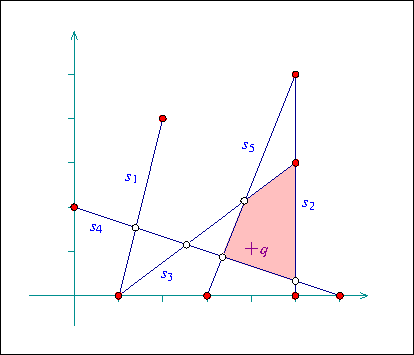
\includegraphics{Arrangement_2/fig/ex_8}
  \end{center}
\end{ccTexOnly}
\begin{ccHtmlOnly}
  <p><center>
  <img src="./fig/ex_8.gif" border=0 alt="Example 8">
  </center>
\end{ccHtmlOnly}
\caption{An arrangement of five intersecting line segments, as
constructed in \ccc{ex_incremental_insertion.C} and
\ccc{ex_aggregated_insertion.C}. The segment
endpoints are marked by black disks and the arrangement vertices
that correspond to intersection points are marked by circles.
The query point $q$ is marked with a cross and the face that
contains it is shaded.\label{arr_fig:ex_8}}
\end{figure}

The program below constructs an arrangement of intersecting
line-segments. We know that $s_1$ and $s_2$ do not intersect, so
we use \ccc{insert_non_intersecting_curve()} to insert them into the
empty arrangement. The rest of the segments are inserted using
\ccc{insert_x_monotone_curve()} or \ccc{insert_curve()}, which are
equivalent in case of line segments. The resulting arrangement consists
of $13$ vertices, $16$ edges, and $5$ faces, as can be seen in
Figure~\ref{arr_fig:ex_8}.

In the earlier examples, all arrangement vertices corresponded to
segment endpoints. In this example we have additional vertices that
correspond to intersection points between two segments. The
coordinates of these intersection points are rational numbers, if
the input coordinates are rational (or integer). Therefore,
the \ccc{Quotient<int>} number type is used to represent the
coordinates:

\ccIncludeExampleCode{../examples/Arrangement_2/ex_incremental_insertion.C}

\subsection{Aggregated Insertion Functions\label{arr_ssec:agg_insert}}
%------------------------------------------

Let us assume that we have to insert a set of $m$ input curves into an
arrangement. It is possible to do this incrementally, 
inserting the curves one by one, as shown in the previous section.
However, the arrangement package provides three free functions that
aggregately insert a range of curves into an arrangement:
%
\begin{itemize}
\item \ccc{insert_non_intersecting_curves(arr, begin, end)} inserts 
a range of $x$-monotone curves given by the input iterators
\ccc{[begin, end)} into an arrangement \ccc{arr}. The $x$-monotone
curves should be pairwise disjoint in their interior and also
interior-disjoint from all existing edges and vertices of \ccc{arr}.
%
\item \ccc{insert_x_monotone_curves(arr, begin, end)} operates on
a range of $x$-monotone curves that may intersect one another.
%
\item \ccc{insert_curves(arr, begin, end)} inserts a range of
of general (not necessarily $x$-monotone) curves of type \ccc{Curve_2},
given by the input iterators \ccc{[begin, end)}, into the arrangement
\ccc{arr}.
\end{itemize}

We distinguish between two cases: (i) The given arrangement
\ccc{arr} is empty (has only an unbounded face), so we have to
construct it from scratch. (ii) We have to insert $m$ input curves
to a non-empty arrangement \ccc{arr}.

In the first case, we sweep over the input curves, compute
their intersection points and construct the \dcel\ that represents
their planar arrangement. This process is performed in
$O\left((m + k)\log m\right)$ time, where $k$ is the total number
of intersection points. The running time is asymptotically better
than the time needed for incremental insertion, if the arrangement
is relatively sparse (when $k$ is bounded by $\frac{m^2}{\log
m}$), but in practice it is recommended to use this aggregated
construction process even for dense arrangements, since the
sweep-line algorithm needs less geometric operations compared to
the incremental insertion algorithms and hence typically runs 
much faster in practice.

Another important advantage the aggregated insertion functions
have is that they do not issue point-location queries. Thus, no
point-location object needs to be attached to the arrangement. As
explained in Section~\ref{arr_ssec:pl}, there is a trade-off
between construction time and query time in each of the
point-location strategies, which affects the running times of the
incremental insertion process. Naturally, this trade-off is irrelevant
in case of aggregated insertion as above.

The example below shows how to construct the arrangement of
line segments depicted in Figure~\ref{arr_fig:ex_8} and built
incrementally in \ccc{ex_incremental_insertion.C}, as shown in the previous
section. We use the aggregated insertion function
\ccc{insert_x_monotone_curves()} as we deal with line segments.
Note that no point-location object needs to be defined and attached to the
arrangement:

\ccIncludeExampleCode{../examples/Arrangement_2/ex_aggregated_insertion.C}

In case we have to insert a set of $m$ curves into an existing
arrangement, where we denote the number of edges in the arrangement by $N$.
As a rule of thumb, if $m = o(\sqrt{N})$, we insert the curves one by
one. For larger input sets, we use the aggregated insertion procedures.

\begin{figure}[t]
\begin{ccTexOnly}
  \begin{center}
  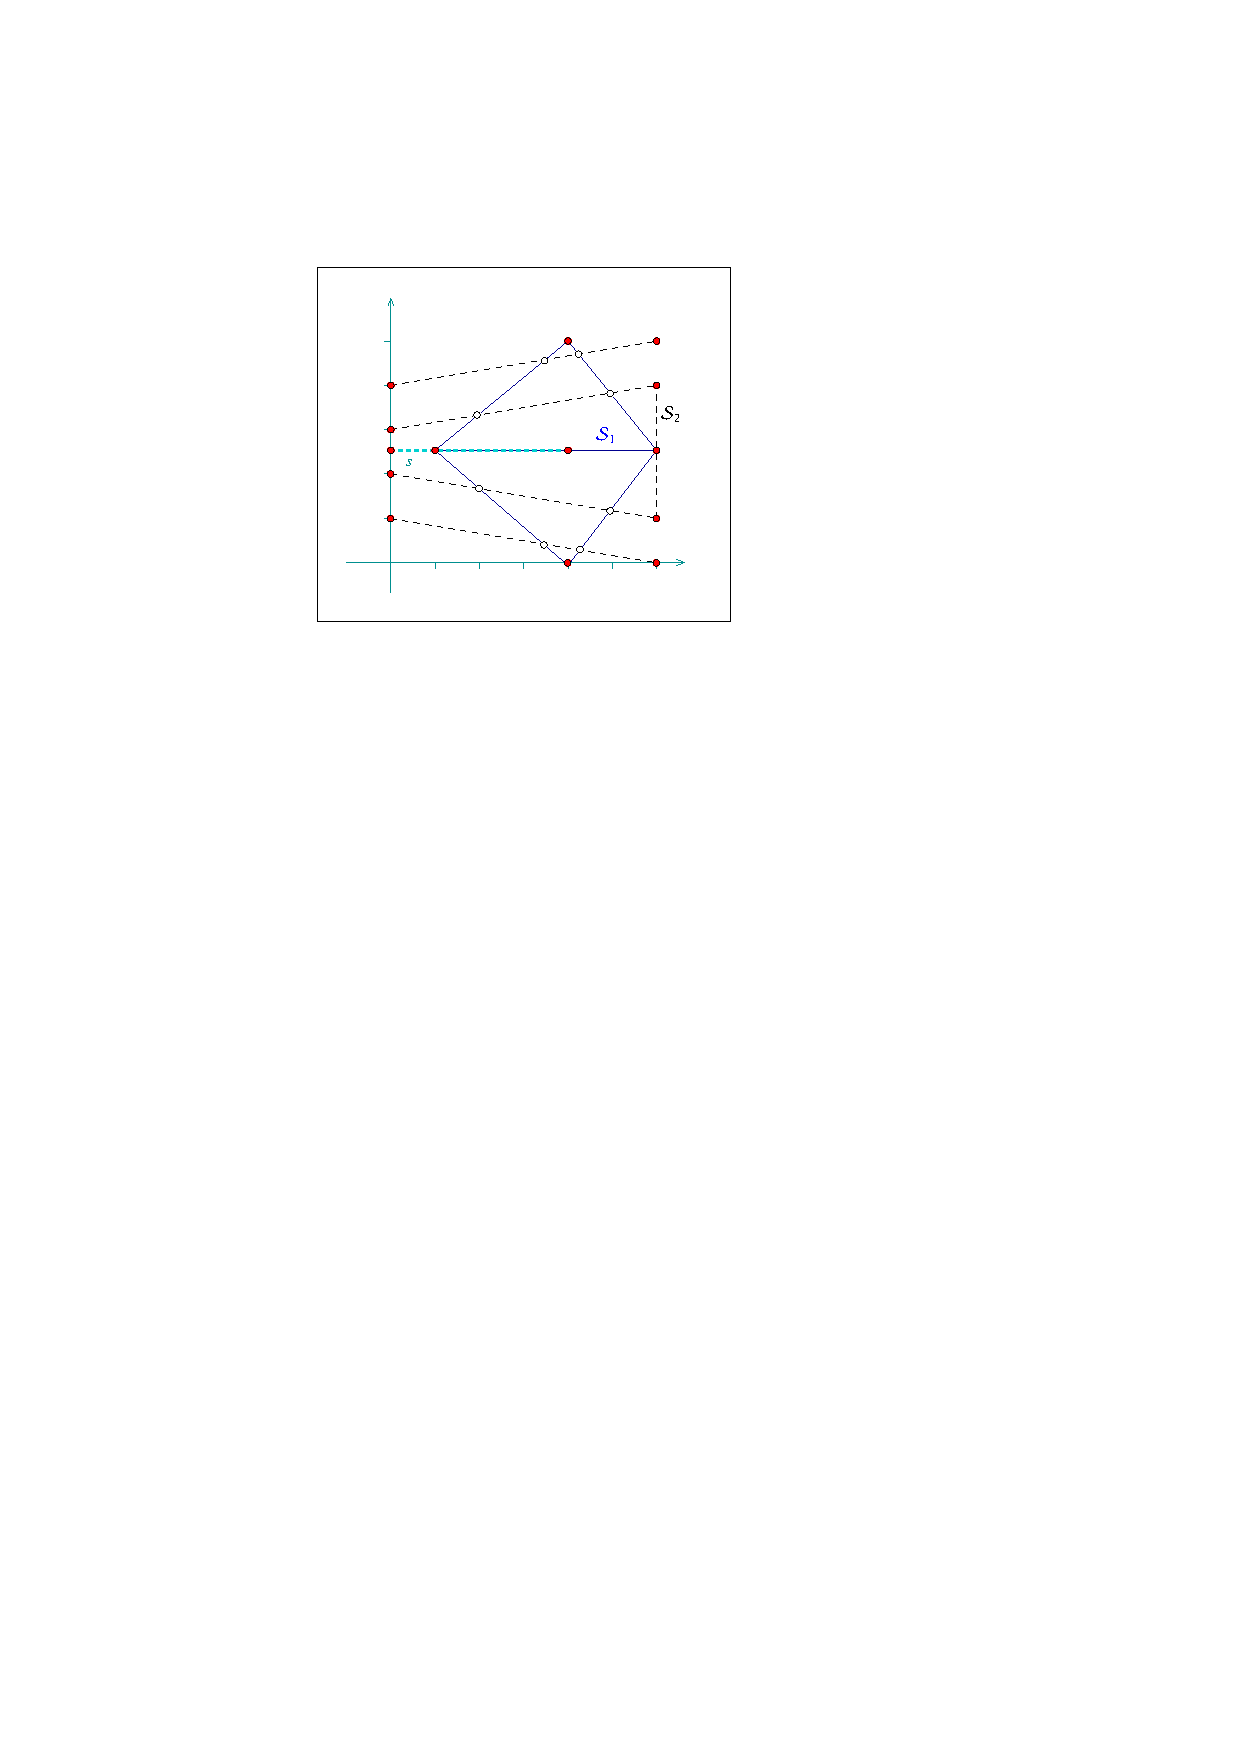
\includegraphics{Arrangement_2/fig/ex_10}
  \end{center}
\end{ccTexOnly}
\begin{ccHtmlOnly}
  <p><center>
  <img src="./fig/ex_10.gif" border=0 alt="Example 10">
  </center>
\end{ccHtmlOnly}
\caption{An arrangement of intersecting line segments, as
constructed in \ccc{ex_global_insertion.C}. The segments of ${\mathcal S}_1$
are drawn in solid lines and the segments of ${\mathcal S}_2$ are
drawn in dark dashed lines. Note that the segment $s$ (light
dashed line) overlaps one of the segments in
${\mathcal S}_1$.\label{arr_fig:ex_10}}
\end{figure}

In the example below we aggregately construct an arrangement of a set
${\mathcal S}_1$ containing five line segments. Then we insert a single
segment using the incremental insertion function. Finally, we add a set
${\mathcal S}_2$ with five more line segments in an aggregated fashion.
Notice that the line segments of ${\mathcal S}_1$ are pairwise
interior-disjoint, so we use \ccc{insert_non_intersecting_curves()}.
${\mathcal S}_2$ also contain pairwise interior-disjoint segments,
but as they intersect the existing arrangement, we have to use
\ccc{insert_x_monotone_curves()} to insert them. Also note that the
single segment $s$ we insert incrementally overlaps an existing
arrangement edge:

\ccIncludeExampleCode{../examples/Arrangement_2/ex_global_insertion.C}

The number type used in the example above,
\ccc{Quotient<MP_Float>}, is comprised of a numerator and a
denominator of type \ccc{MP_Float}, namely floating-point numbers
with unbounded mantissa. This number type is therefore capable of
exactly computing the intersection points as long as the segment
endpoints are given as floating-point numbers.

\subsection{Removing Vertices and Edges\label{arr_ssec:gl_remove}}
%---------------------------------------

The free functions \ccc{remove_vertex()} and \ccc{remove_edge()} handle
the removal of vertices and edges from an arrangement. The difference
between these functions and the member functions of the \ccc{Arrangement_2}
template having the same name is that they allow the merger of two curves
associated with adjacent edges to form a single edge. Thus, they require
that the traits class that instantiates the arrangement instance is a model
of the refined \ccc{ArrangementXMonotoneTraits_2} concept (see
Section~\ref{arr_sec:traits}).

The function \ccc{remove_vertex(arr, v)} removes the vertex
\ccc{v} from the given arrangement \ccc{arr}, where \ccc{v} is
either an isolated vertex or is a {\em redundant} vertex ---
namely, it has exactly two incident edges that are associated with
two curves that can be merged to form a single $x$-monotone curve.
If neither of the two cases apply, the function returns an
indication that it has failed to remove the vertex.

The function \ccc{remove_edge(arr, e)} removes the edge \ccc{e}
from the arrangement by simply calling \ccc{arr.remove_edge(e)}
(see Section~\ref{arr_ssec:modify}). In addition, if either of the
end vertices of \ccc{e} becomes isolated or redundant after the removal
of the edge, it is removed as well.

\lcTex{%
  \setlength{\ArrangementTwoWidthRight}{1.5cm}
  \setlength{\ArrangementTwoWidthLeft}{\ArrangementTwoWidthLineReal}
  \addtolength{\ArrangementTwoWidthLeft}{-\ArrangementTwoWidthRight}
  \begin{minipage}{\ArrangementTwoWidthLeft}
}
\begin{ccHtmlOnly}
  <p><center>
    <img src="./fig/h_shape.gif" border=0 alt="h_shape" align=right>
  </center>
\end{ccHtmlOnly}
The following example demonstrates the usage of the free removal
functions. In creates an arrangement of four line segment forming
an H-shape with a double horizontal line. Then it removes the two
horizontal edges and clears all redundant vertices, such that the
final arrangement consists of just two edges associated with the
vertical line segments:
\lcTex{%
  \end{minipage}\hspace{\ArrangementTwoMinipageSpace}
  \begin{minipage}{\ArrangementTwoWidthRight}
    \begin{center}
    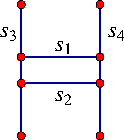
\includegraphics{Arrangement_2/fig/h_shape}
    \end{center}
  \end{minipage}
}

\ccIncludeExampleCode{../examples/Arrangement_2/ex_global_removal.C}
